\chapter{Back-end design}
This chapter describes the communication between server and client, as well as the design choices and
implementation of database. \todo{Bør database være et kapitel for sig selv?}

\section{Communication}
\label{sec:com}

The communication between the client application and the server is done by HTTP POST requests.
The client sends a HTTP POST request to the server containing a certain list of parameters which
define what the server is supposed to do. All requests must take at least two required parameters, a \textit{RequestCode} and a
\textit{Type}.

\textit{RequestCode} is an integer that is simply passed through the server, it is not handled in any
way on the server. The purpose of the RequestCode parameter is to distinguish the request on the client allowing
it to execute the appropriate function.

\textit{Type} is used to identify the request. A typical request is to get a list of feeds, and the
value of the \textit{Type} parameter would be ``GetFeeds'' in this case.

Depending on the \textit{Type} of the request, additional parameters may be required. As an example, \textit{GetFeeds} takes the following parameters:
\begin{itemize}
\item RequestCode
\item UserId
\item Limit
\end{itemize}

The approach is to process the request on the serverside, and make the right calls to the
database. The server will then return a JSON object containing all the relevant information that was
requested. This JSON object can easily be parsed on the client side. The reason why we chose JSON as
a format is because it is well supported and easy to generate in both android and PHP.

\begin{lstlisting}[language=phpstyle, caption=getFeeds function call]
$requestCode = $_POST["RequestCode"];

switch ($_POST['Type']) {
        case "GetFeeds":
            getFeeds($con, $_POST['UserId'], $_POST['Limit']);
            break;
}
\end{lstlisting}

\begin{description}
\item[Line 1] Get the \textit{RequestCode} parameter.
\item[Lines 3-7] If \textit{Type} equals ``GetFeeds'', call the getFeeds function.
\end{description}

\todo{Nævn de andre cases, måske her?}

\begin{lstlisting}[language=phpstyle, label=lst:getFeeds, caption={getFeeds function}]
function getFeeds($con, $userId, $limit) {

    global $requestCode;

    #Escape special characters to avoid SQL injection attacks
    $userId    = $con->real_escape_string($userId);
    $limit     = $con->real_escape_string($limit);

    $query =   "SELECT feeds.id, feeds.boothid, feeds.header, feeds.description, feeds.feedtime, userbooths.userid, companies.logo, booths.name ".
        "FROM feeds ".
        "LEFT JOIN userbooths ".
        "ON feeds.boothid = userbooths.boothid ".
        "LEFT JOIN booths ".
        "ON feeds.boothid = booths.id ".
        "LEFT JOIN companies ".
        "ON booths.companyid = companies.id ".
        "WHERE userid = ".$userId." ".
        "AND sub = 1 ".
        "ORDER BY feeds.feedtime DESC ".
        "LIMIT "$limit;

    $result = $con->query($query);

    $json = array();
    while($row = $result->fetch_object()) {
      array_push($json, $row);
    }
    
    $final->RequestCode = $requestCode;
    $final->Data = $json;
    echo json_encode($final);
}
\end{lstlisting}

\begin{description}
\item[Line 1] The function takes three parameters, the MySQLi object which has a connection
  established to the database, the user id from the client, and the limit which is also given by the client.
\item[Line 3] Since the \textit{RequestCode} is always a required parameter the variable is global.
\item[Lines 6-7] Escape special characters to avoid malicious SQL injections.
\item[Lines 9-20] Create the SQL query with the user id and the limit parameter.
\item[Line 22] Execute the query.
\item[Lines 24-31] Get the results from the database and push them to the JSON array. When
  all of the results have been pushed to the array, the \textit{RequestCode} and the JSON array will be JSON encoded and echoed.
\end{description}

As seen on line 29 in \autoref{lst:getFeeds} the result is JSON encoded and then echoed. An example of a result from the \textit{GetFeeds} type request could look like the following:

\begin{lstlisting}[language=json, label=lst:jsonResult, caption=Example result from a request with type: \textit{GetFeeds}]
{
    "RequestCode": "1",
    "Data": [
        {
            "id": "16",
            "boothid": "90",
            "header": "Windows 9",
            "description": "Come and get a preview of the new Windows 9!",
            "feedtime": "2013-11-21 13:39:20",
            "userid": "66",
            "logo": "microsoftlogo.png",
            "name": "Gruppe nr 5"
        },
        {
            "id": "1",
            "boothid": "90",
            "header": "Welcome to the exhibition!",
            "description": "Welcome to this test exhibition, we hope you enjoy your stay.",
            "feedtime": "2013-11-21 13:17:36",
            "userid": "66",
            "logo": "microsoftlogo.png",
            "name": "Gruppe nr 5"
        }
    ]
}
\end{lstlisting}

Note that the result in \autoref{lst:jsonResult} is an object with two attributes, the data and the request code. The result will always be in this format.

All of the requests to the server follows this principle. A request is made, the query is run and data is gathered, and lastly the result is returned as a JSON object that the client reads.\\\\
Our types of requests are as follows:
\begin{itemize}
\item \textbf{GetFeeds}\\
 Will return all the necessary data about a certain number of feeds. They are sorted to return the newest feed first and then the next number of feeds that corresponds to the given limit parameter.
\item \textbf{CreateUser}\\
  Creates a new user in the database and returns the userid.
\item \textbf{GetNewFeeds}\\
  Returns data about all new feeds since the last update. This means that the user can manually fetch all new feeds.
\item \textbf{CheckFeeds}\\
  Check if any new feeds are available, and if such the number of new feeds will be returned.
\item \textbf{GetOldFeeds}\\
  Load a certain number of feeds that are older than the current oldest feed showing. This allows the user to load the next batch of feeds.
\item \textbf{GetSchedule}\\
  Returns relevant data about the schedule of the exhibition. Used for the schedule tab on the android application.
\item \textbf{GetExhibitionInfo}\\
  Returns all information about the exhibition, such as the description and logo.
\item \textbf{GetCategories}\\
  Returns a list of categories, and the booths of this category, that are associated with the current exhibition. It also contains a flag that shows whether the user is currently subscribed to a booth or not.
\item \textbf{SetCategories}\\
  This request is run when the ``submit'' button is pressed in the category chooser. This updates the booths that the user is subscribed to in the database.
\end{itemize}

\section{Database}
We are using a MySQL database with the MyISAM storage engine and which is located at a remote server. \todo{info om hvor osv.?}

The server contains all data about each exhibition, the companies at the exhibition, the feeds, the schedule, and some basic information about the users.

\autoref{fig:erd} shows the \ac{er} diagram of our database. The diagram does not show the attributes of the entities in order to make the diagram a little smaller.

\begin{figure}[H]
\centering
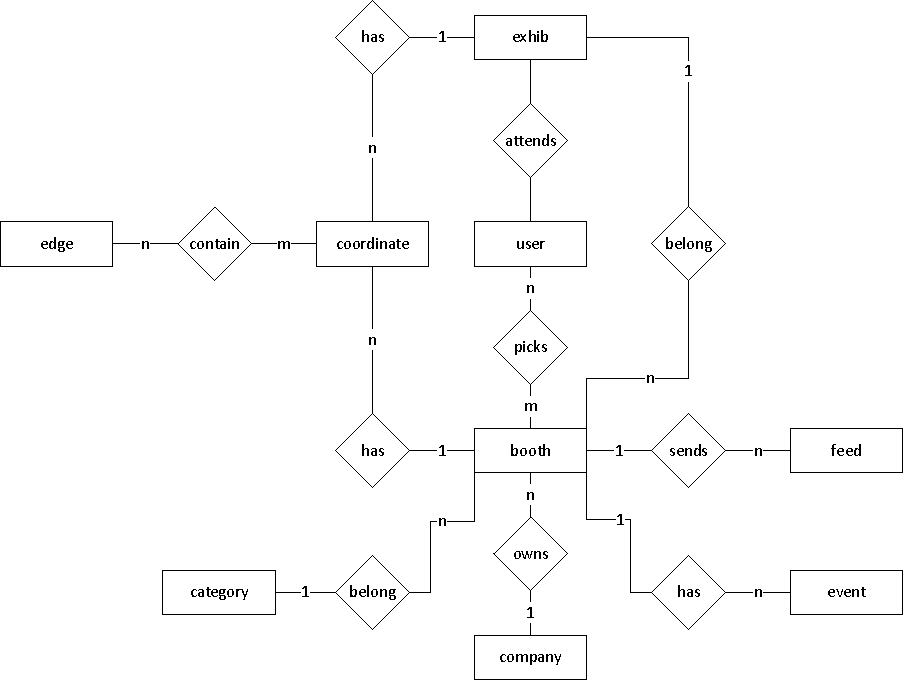
\includegraphics[page=1,width=1\linewidth]{img/sw7ERD.pdf}
\caption{ER diagram}
\label{fig:erd}
\end{figure}

\newcommand{\rel}[2]{$(#1:#2)$}

Some of the relationships in the \ac{er} diagram needs a little detailed description, but most of them are self explanatory.

All functional relationship types are total participations, except for the relationship \textit{has} between \textit{coordinate} and \textit{booth}, which is partial participation.

The \textit{attends} relationship between \textit{exhib} and \textit{user} is a \rel{1}{n} because we decided that one person that attends different exhibitions will get a new user for each exhibition he visits. We could also have made it an \rel{n}{m} relationship, but that would require us to make some kind of way to retrieve an existing user for that person and then also subscribe him to that exhibition. The user is not required to give any information when he is registered to an exhibition i.e. the registration is automatic, then we do not need to save any user data to be used at other exhibitions.

The \textit{contain} relationship between edge and \textit{coordinate} is shown to be a \rel{n}{1}, but the \textit{edge} actually contains exactly two coordinates, which can not be shown with Chen notation.

\textit{Category} only has a relationship with \textit{booth}. This means that one specific category can be used for multiple booths at different exhibitions. This is a design choice.

\autoref{tab:relations} shows the mapping of our \ac{er} diagram to relations.

\newcommand{\relation}[1]{[\{ #1 \}]\\}

\begin{table}[H]
\centering
\small
\begin{tabular}{p{1.2cm} p{9.6cm}}
booth: & \relation{\underline{id: int}, exhibid $\ra$ exhib: int, categoryid $\ra$ category: int, companyid $\ra$ company: int, name: varchar, description: text}
category: & \relation{\underline{id: int}, name: varchar}
company: & \relation{\underline{id: int}, name: varchar, logo: varchar}
coordinate: & \relation{\underline{id: int}, x: double, y: double, isroad: tinyint, boothid $\ra$ booth: int, exhibid $\ra$ exhib: int}
edge: & \relation{\underline{id: int}, weight: double, vertexA $\ra$ coordinate: int, vertexB $\ra$ coordinate: int}
exhib: & \relation{\underline{id: int}, name: varchar, address: varchar, zip: int, country: varchar, description: text, logo: varchar}
feed: & \relation{\underline{id: int}, boothid $\ra$ booth: int, header: varchar, description: text, feedtime: timestamp}
schedule: & \relation{\underline{id: int}, boothid $\ra$ booth: int, name: text, starttime: timestamp, endtime: timestamp}
picks: & \relation{\underline{id: int}, userid $\ra$ user: int, boothid $\ra$ booth: int, seen: tinyint, sub: tinyint}
user: & \relation{\underline{id: int}, exhibid $\ra$ exhib: int}
\end{tabular}
\caption{Relations}
\label{tab:relations}
\end{table}
\todo{why zip == int?}
\todo{Måske skriv at vi ikke kan bruge foreign keys i vores database}
A coordinate can be of three different types. If \textit{boothid} is null and \textit{isroad} is not null the coordinate is simply a point on the road. If \textit{boothid} is not null and \textit{isroad} is null the coordinate is a point used to define where the booth lies. If neither of the two attributes are null the coordinate is an entrance to the booth, i.e. the point lies on the road but is a part of the booth.
%%% Local Variables: 
%%% mode: latex
%%% TeX-master: "../master"
%%% End: 
